%% Based on a TeXnicCenter-Template by Tino Weinkauf.
%%%%%%%%%%%%%%%%%%%%%%%%%%%%%%%%%%%%%%%%%%%%%%%%%%%%%%%%%%%%%

%%%%%%%%%%%%%%%%%%%%%%%%%%%%%%%%%%%%%%%%%%%%%%%%%%%%%%%%%%%%%
%% PDF-Informations
%%%%%%%%%%%%%%%%%%%%%%%%%%%%%%%%%%%%%%%%%%%%%%%%%%%%%%%%%%%%%
%%
%% ATTENTION: You need a main file to use this one here.
%%            Use the command "\input{filename}" in your
%%            main file to include this file.
%%

\pdfinfo{                               % Info dictionary of PDF output;
                                        % all keys are optional.
    /Author (Virgile Lebailly)
    /CreationDate (D:20011010111111)    % (D:YYYYMMDDhhmmss)
                                        % YYYY  year
                                        % MM    month
                                        % DD    day
                                        % hh    hour
                                        % mm    minutes
                                        % ss    seconds
                                        %
                                        % default: the actual date
                                        %
    /ModDate (D:20011010111111)         % ModDate is similar
    /Creator (TeX && TXC)               % default: "TeX"
    /Producer (pdfTeX)                  % default: "pdfTeX" + pdftex version
    /Title (Cahier des charges)
    /Subject ()
    /Keywords ()
}

\documentclass{report}

\usepackage[latin1]{inputenc}  %pour pouvoir utiliser tous les caract�res de mon clavier
\usepackage[T1]{fontenc}   %idem
\usepackage[francais]{babel}  %pour sp�cifier que j'�cris en francais
\usepackage{makeidx}
\usepackage{graphicx}
\usepackage{array}

\title{Varou}
\author{Dreams Makers}
\date{16 Mars 2015}

\makeindex
\begin{document}

\maketitle

\tableofcontents


Projet Varou


Game Design Document


Une production Dreams makers

\part{Introduction}

	\chapter{Informations g�n�rales}
		\section{Description du jeu}
Varou est un jeu d'aventure/RPG � la Zelda. La partie RPG ne concerne pas le personnage, qui n'�voluera pas, mais le fait que chaque d�cision prise influencera la suite de l'histoire. Le joueur dirigera le personnage et devra g�rer son �quipement de plus les combats seront en temps r�el.
Il poursuivra une qu�te principale et aura une multitude de qu�tes secondaires qui pourront influer sur la qu�te principale.

Le principe de Varou est celui de la plupart des jeux d'aventure. Notre personnage devra accomplir une qu�te, traverser les contr�es glauques, r�soudre des �nigmes et biensur de combattre des ennemis. Le jeu prend place dans un univers � la fois vampirique, ambiance transylvanie et � la fois un univers steampunk. Que ce soit dans les villes, en campagnes, dans les batiments, le personnage peut parler aux PNJ, les attaquer, acheter et vendre des objets aux personnes ad�cquats. Il peut int�ragir avec l'environnement, mais cela peut se faire au d�triment de la popularit� aupr�s des PNJs.

\section{Cat�gorisation du jeu}
RPG
\section{Public vis�}
Fan steampunk, averti, ...
\section{Les Trois piliers qui soutiennent le jeu}
Un piler = id�e g�niale ou presque, originale, ...

\part{Design du jeu}

	\chapter{Histoires}
		\section{R�sum�}
Truc de 15 lignes, avec les principales �tapes.
\section{Personnage principal}
C'est qui, d'o� il vient, etc.
	
	\chapter{Frontend}
		\section{Gameplay}
	\subsection{D�placements}
	\subsection{En combat}
	Le syst�me de combat de Varou est du hack and slash. C'est � dire que l'on devra cliquer pour taper avec l'arme choisi. Le clic droit servira quand � lui � se servir de son 		environnement, le temps ralentissant quand l'on est dans le menu. La souris �tant libre. L'environnement �tant dynamique, le joueur devra se placer et int�ragir intelligement 	 pour gagner ses combats.
\section{Int�raction avec l'environnement}

	\subsection{Int�raction avec les PNJs}

	\subsection{Int�raction avec les objets}

\section{GUI}

\section{Style graphiques}
	Ambiance, palette de couleur, etc.
\section{Style musical et bruits d'ambiance}

\part{M�caniques}
	\chapter{Crafts}
		\section{Sur place}
	trucs que l'on peut faire n'importe o�
	\section{A emporter}
	Necessite la presence d'un element fixe, un pnj, un batiment, ...
		
	\chapter{Techniques et aptitudes}
		blabla
		
	\chapter{Combat et calculs des d�g�ts}
		blabla
		
	\chapter{Magie}
		Magie
	
	\chapter{Glyphs}
		Glyphs	
	
	\chapter{Qu�tes}
		Quetes
	
	\chapter{Inventaire}
		Inventaire
	
	\section{Gestion de l'inventaire du h�ro}
		Inventaire
	
	\section{Marchants}
		Inventaire	
	
	\chapter{Interactions avec l'environnement}
		interraction environnement	
	
	\chapter{V�ttfang}
		\section{Mat�riel}
Ce jeu se joue avec un deck de 50 cartes et un sceau de 100 d�s.\\
Il � un tapis de jeu de 5 emplacements de cartes par joueurs.

\section{R�gles}

Au d�but de la partie, chaque joueur choisi un nombre de d� (cach�) dans sa r�serve. Celui qui obtient le plus haut score joue en deuxi�me.\\
Les tours sont divis�s en 3 phases :
		\begin{itemize}
				\item Phase de pioche :\\
				Le joueur pioche jusqu'� avoir 5 cartes en main.
				\item Phase de pose :\\
				Le joueur pose ses cartes et peut d�placer une seule carte.
				\item Phase d'attaque :\\
				Le joueurs peut attaquer avec une cr�ature. Une carte ne peut attaquer que la carte en face d'elle.
		\end{itemize}
		
La phase d'attaque est divis�e en plusieurs sections :
		\begin{itemize}
				\item Le joueur attaquant d�clare avec qu'elle carte il va attaquer
				\item Le joueur attaquant d�clare combien de d�s il va utiliser pour attaquer
				\item Le joueur d�fenceur d�clare combien de d�s il va utiliser pour d�fendre
				\item Le joueur attaquand d�clare combien de d�s il va utiliser pour son pari
				\item R�solution du combat
		\end{itemize}

\section{pari}
	Le joueur attaquant peut placer un pari sur son attaque.\\
	Pour cela le joueur doit consommer des d�s de sa r�serve pour pouvoir gagner un multiplicateur de score. Attention, si le joueur perd le combat, le multiplicateur est aussi
	utilis�.\\
	Le joueurs attaquant peut utiliser jusqu'� 5 d�s, mais pas plus de d�s qu'il n'y a de cartes en jeu.
			\begin{itemize}
				\item 1 d�  : x2
				\item 2 d�s : x4
				\item 3 d�s : x8
				\item 4 d�s : x16
				\item 5 d�s : x32
		\end{itemize}
		
\section{Cartes}
Les cartes ont plusieurs attribus :
		\begin{itemize}
				\item Nom : Le nom de la carte
				\item Valeur : La valeur de la carte (sa puissance)
				\item Co�t : Le co�t en points de la carte pour la poser
				\item Co�t � vide : Le co�t en points de la carte si le joueur n'a aucune carte en jeu
				\item Attaque : La valeur d'attaque de la carte
				\item D�fense : La valeur de d�fense de la carte
				\item Capacit� : La capacit� de la carte si elle en poss�de une
		\end{itemize}
		
\section{Pose des cartes}
Le joueur dont c'est le tour peut poser jusqu'� 5 cartes devant lui.\\
Pour cela il doit soustraire de son score le co�t en points de la carte.

\section{Combat}
Pour savoir qui gagne le combat :\\
(Attaque de la carte + r�sultat des d�s) = Vatt\\
(D�fense de la carte + r�sultat des d�s) = Vdef\\
\\
Vatt VS Vdef\\
\\
Si l'attaquant gagne, la carte d�fenseur est tu�e.\\
Et l'attaquant augmente son score de :\\
(((Vatt - Vdef)/nombre de d�s utilis�s)+(Valeur de la carte d�fensive - Valeur de la carte attaquante))*multiplicateur de pari\\
\\
Si l'attaquant perd, aucune carte n'est tu�e � moins que la diff�rence de combat ne soit sup�rieur � la d�fense de la carte attaquante. Dans ce cas celle-ci est d�truite.\\
Et l'attaquant diminue son score de :\\
(((Vdef - Vatt)*nombre de d�s utilis�s)+(Valeur de la carte attaquante - Valeur de la carte d�fensive))*multiplicateur de pari\\
\\
Un score ne peut jamais �tre n�gatif\\

\section{fin de partie}
La partie prend fin si un joueur n'a plus de d�s dans sa r�serve au d�but de son tour.\\
OU\\
La partie prend fin si un joueur n'a plus de carte dans son deck ni en jeu � la fin de son tour.\\
Le joueur ayant le meilleur score remporte la partie.

\section{Graphismes}
Voir le sceau de d� diminuer quand on y pioche des d�s et qu'on puisse les compter quand on arrive � la fin.\\
On ne voit pas combien de d�s il reste � l'adversaire (m�me � la fin)

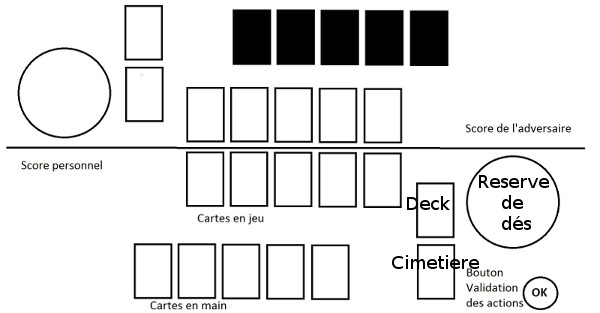
\includegraphics{T3_Mecaniques/Cartes&Des_Images/Plateau_de_jeu.jpg}

\section{liste des cartes}

\begin{tabular}{|c|c|c|c|c|c|}
	\hline
  Nom & Valeur & Co�t (Co�t � vide) & Attaque & D�fense & Capacit� \\
  \hline
  \hline
  Paysan & 1 & 20 (0) & 6 & 6 & - \\
  \hline
  Marchant & 1 & 20 (0) & 5 & 7 & - \\
  \hline
  Bucheron & 2 & 50 (0) & 8 & 7 & - \\
  \hline
\end{tabular}	

\part{Level design}

\chapter{IV.1_

\part{Outils}

\chapter{V.1 GitHub}
		\section{Description}
GitHub est un outil permettant de travailler � plusieurs sur un projet et plus particuli�rement sur un ensemble de fichiers synchronis�s.
Le d�p�t utilis� est situ� � https://github.com/pakoskyfrog/Varou
\section{Utilisation}
L'utilisateur doit installer le client et importer le depot.
Avant de se mettre au travail, l'utilisateur doit synchroniser son dossier de travaille afin de poss�der les derni�res modifications.
Durant son travail, � chaque �tape majeure, l'utilisateur devra faire un ��commit��, op�ration qui dit au gestionnaire de GitHub de pr�parer une synchronisation des fichiers.
A la fin de sa session de travail, l'utilisateur devra ��publier�� afin de mettre � jour le d�p�t online avec son travail.
		
\chapter{Wiki}
		Wiki
		
\chapter{Moteur 3D}
		Ogre

	
\end{document}